\section{Mission Design}
\label{sec:mission-design}
% \textcolor{blue}{Contribution (1): "We present remote sensing strategies that augment the capabilities of pushbroom hyperspectral imaging with particular application for HYPSO-1. Given the constraints using COTS-based optics and sensor in a small-satellite, these strategies entail the spacecraft performing a slew maneuver while imaging to increase Ground Sampling Distance (GSD), SNR and effective spatial resolution in the image pixels. These Figure-of-Merits (FoMs) may be chosen as system-drivers for preliminary system design and may be included in trade-off studies in payload design, thus enabling better performance and capacity for smaller sensor systems." Key points to keep in mind while writing this section:
% \begin{itemize}
%     \item What are the ocean color requirements?
%     \item why is pushbroom hyperspectral imaging good?
%     \item what is the proposed CONOPS to fulfill the requirements and give end users what they want?
%     \item what are the suggested operational modes?
%     \item what trade-offs are accepted?
% \end{itemize}}
\begin{figure*}[htbp]
  \begin{center}
    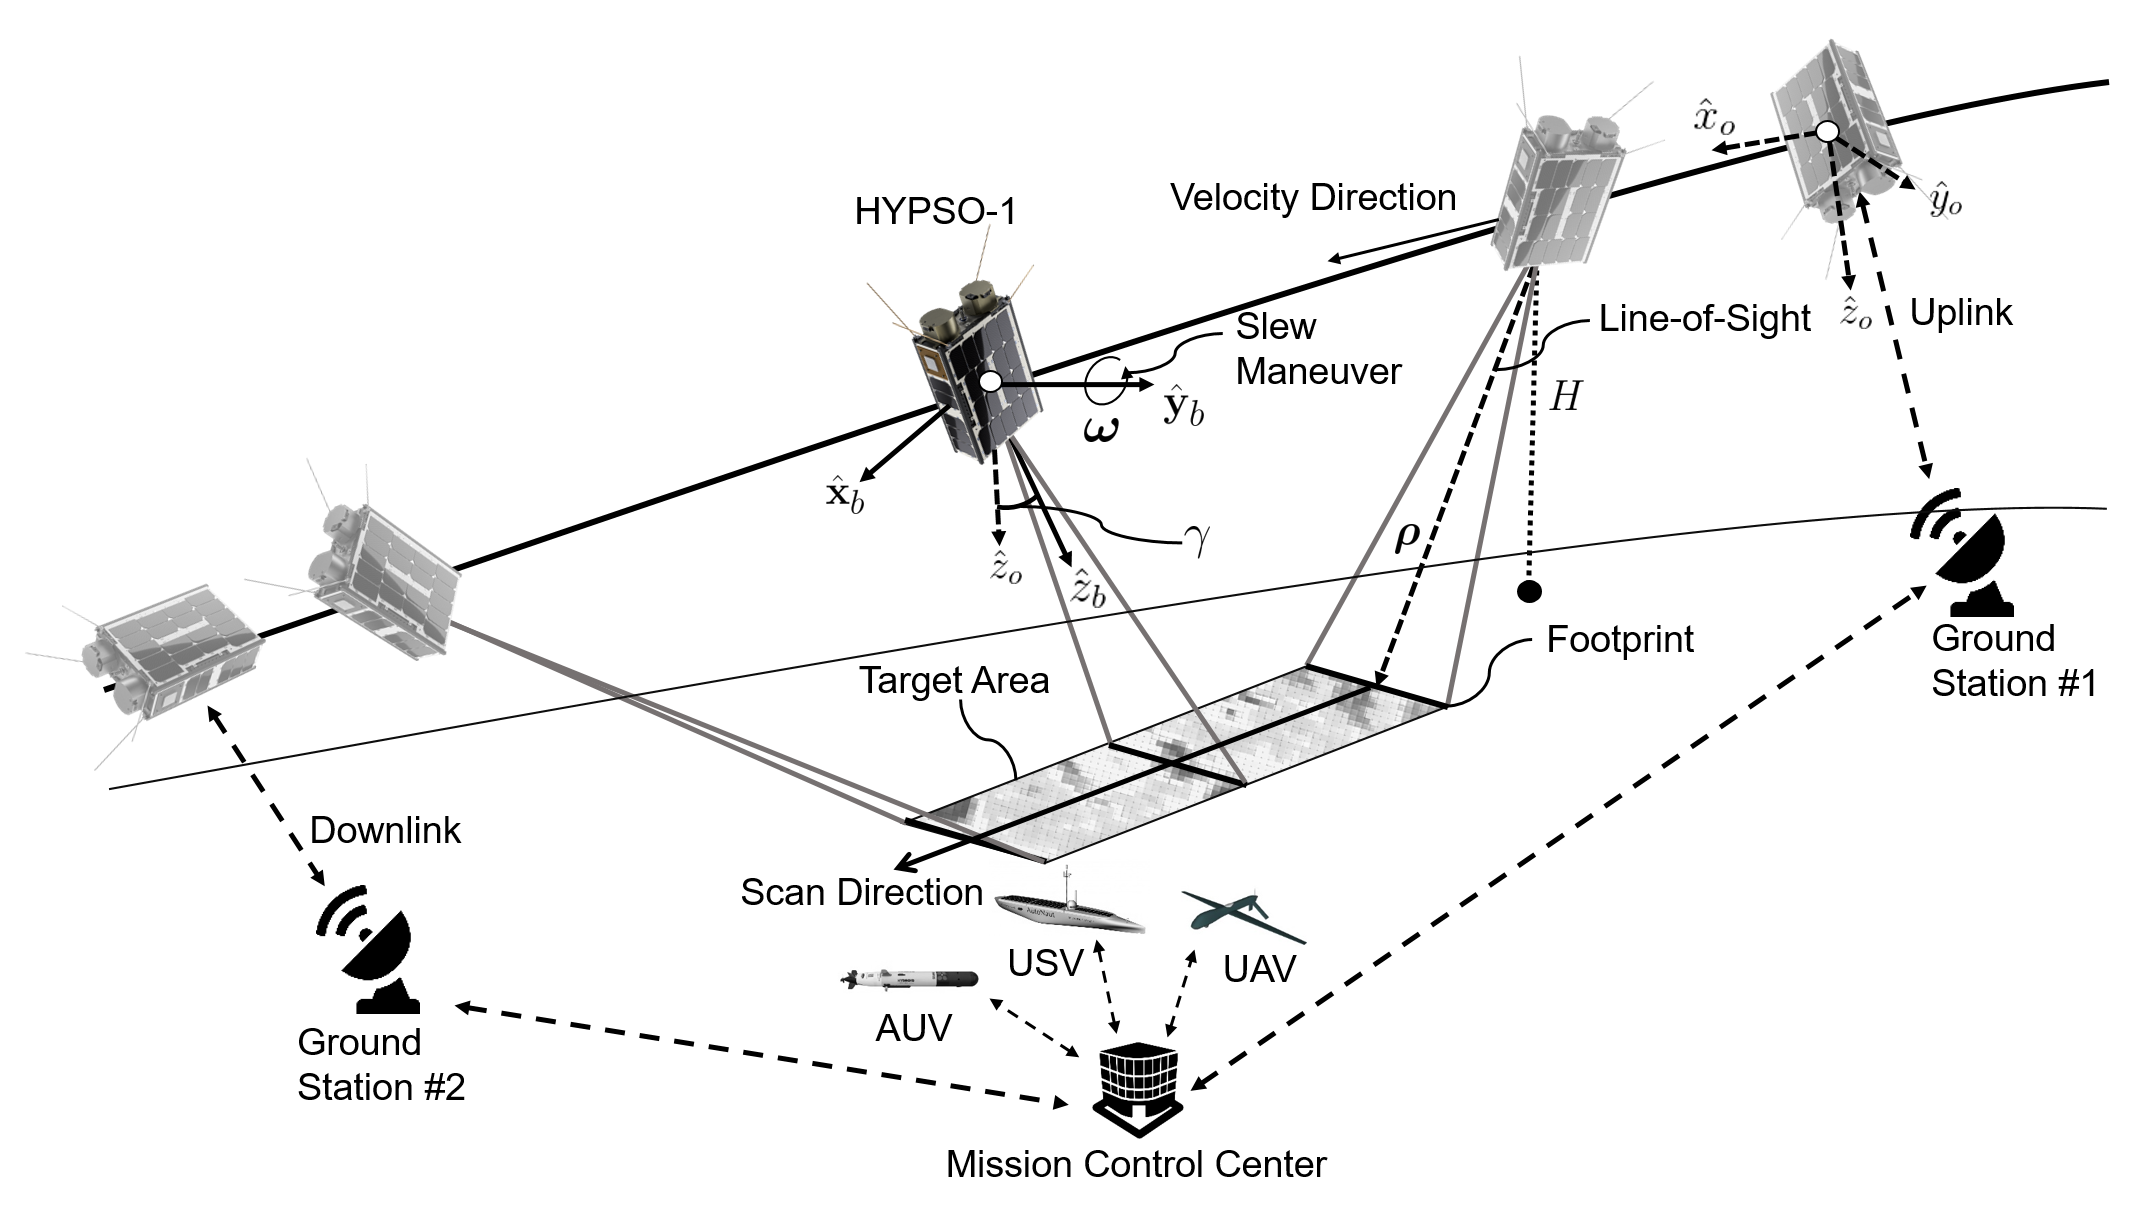
\includegraphics[width=160mm,angle=0]{figs/CONCEPT_HYPSO1.png}
    \caption{HYPSO-1 concept of operations}
    \label{fig:conops}
\end{center}
\end{figure*}
% \subsection{Requirements}\label{sec:requirements}
% \hl{Mariusz \\}
\subsection{Requirements}
In effort to support environmental monitoring, climate research and marine resource management, the objectives of the HYPSO-1 mission are to detect and monitor the spatial extent and motion of algal blooms; characterizing primary productivity; and observing other substances resulting from aquatic habitats as well as water pollution. Based on \cite{Ack16,Dic05, Mouroulis1998, Lancheros2018}, the key recommendations for ocean color remote sensing are:
\begin{enumerate}
    \item Image resolution should be better than $100 \hspace{3pt} \rm{m/pixel}$;
    \item Spectral resolution should be better than $10 \hspace{3pt} \rm{nm}$;
    \item SNR at Top of Atmosphere (ToA) should be greater than $ 100$;
    \item Data should be delivered to end users in less than 12 hours in general and less than 3 hours for HABs; and
    \item Revisit times to target should be at least 3 per day.
\end{enumerate}
Since HYPSO-1 mission is a single small-satellite but the first in a prospective constellation, we focus on working towards satisfying the recommendations 1), 2), 3) and 4). For 5), even though observations of the same target area in consecutive passes are possible, image quality is poor when viewing at large off-nadir angles thus mandating a constellation with multiple satellites to enable many revisits.
%We note that (5) may be artificially achieved if HYPSO-1 data is immediately combined with data from traditional satellites (e.g. Sentinel-3). 
% 
% The inference on algal blooms, especially if harmful, is typically not imminent from solely optical remote sensing \cite{IOCCG2014,IOCCGRep8}, requiring 
% simultaneous or near real-time in-situ measurements that provide data to identify/confirm the algae properties as well as estimating their propagation due to ocean currents and expansion/reduction in spatial extent. 

Monitoring the ocean from space requires cameras that capture enough light because the Earth's atmosphere weakens and scatters the water-leaving radiance \cite{Davis:02}, and most of the phytoplankton and algae typically reside at $10-15 \hspace{3pt} \rm{m}$ below the water surface \cite{IOCCG2014}. Such dark targets normally need tailored atmospheric correction schemes to retrieve the actual ground reflectance in the data \cite{Corson2008, Gao2009}.
% Furthermore, to mitigate the sun-glint effects that obscure the water-leaving radiance, observations should be made when solar zenith angle at the target is between $30-60 \hspace{3pt} \rm{deg}$ and the camera is tilted at an off-nadir viewing angle of $40 \hspace{3pt} \rm{deg}$ and sun-angle of $135 \hspace{3pt} \rm{deg}$ \cite{Kay2009}. 
\subsection{Imaging Trade-offs}
Many spectrometers can be integrated on aerial or space platforms \cite{Mouroulis2018, Wolfe1997}. In particular the pushbroom imager design is an attractive choice. It is able to obtain relatively good SNR since the hosting satellite moves in an approximately local linear track while the imager sequentially captures lines of cross-track pixels, each instantaneously contains dozens or hundreds of narrow spectral bands \cite{Fowler2014, VANE1993127}. 
  
From an orbit altitude, small sensor systems on small-satellites typically provide low instantaneous spatial resolution and SNR. A flexible performance factor and work-around is to improve the Sequential Ground Sampling Distance (SGSD). Here SGSD is taken to be the Euclidean distance between the centers of a reference pixel as seen from ground in two consecutive frames rather than the instantaneous ground distance between adjacent pixels which is commonly defined as the Ground Sampling Distance (GSD). The SGSD may be decreased by tilting the sensor or whole spacecraft while the camera is capturing images. This results in increased number of partially overlapping pixels that may be utilized by super-resolution techniques to improve the SNR and spatial resolution. 

Moreover, a suitable objective is be to map small specific target area(s) of interest that may be quickly revisited. This enables the use of an imaging system with high spectral resolution, a relatively narrow Field-of-View (FoV) and high camera frame rate which do not excessively compromise the SNR nor produce excessive amount of data to downlink. 
\subsection{Concept of Operations}
% Field campaigns with existing AUVs, that are sampling chl-a and characterizing ocean substances in the upper water column, are organized regularly in the Fr{\o}ya region in Mid-Norway, Western Norway as well as Svalbard \cite{Fossum19,fossum18,fossum18b}. The HYPSO-1 mission may provide the necessary macro-perspective and may alert ground operators to investigate specific areas of interest to support these campaigns. The existing AUVs and other assets that give point-to-point in-situ measurements or ground truth, such as from USVs and UAVs, shall be utilized for vicarious calibration and validation of the hyperspectral data \hl{[ref]}.
\begin{figure}[htbp]
  \begin{center}
    
\includegraphics[width=70mm,angle=0]{figs/trade-off chart.png}
    \caption{Diagram showing trade-offs. The extent of the gray pointers indicate the importance of each trade-off at the vertices. "$\otimes$" corresponds to favoured placement of the overall design selection.}
    \label{fig:trade-off}
\end{center}
\end{figure}
HYPSO-1 shall be launched into Sun-Synchronous Orbit (SSO) at an altitude of approximately $500 \hspace{3pt} \rm{km}$ and a LTAN/LTDN between 10:00-11:00 AM. The chosen orbit grants access to observe the Norwegian coastline in the morning during Spring and Summer seasons and also supports the local field campaigns. The particular choice of orbit is chosen as a trade-off between mainly the footprint size, image resolution, SNR, data latency and coverage to selected ground stations and target areas, as seen in Figure \ref{fig:trade-off}. Moreover, the advantage of SSO is that the satellite passes over any given point on the Earth’s surface at approximately the same local sidereal time. Combined with appropriate viewing angles during imaging, the observation windows are also safe from detrimental sun-glint effects \cite{Kay2009}.
% Because ocean color phenomena such as primary productivity are more prevalent in the morning or mid-day, the launch LTAN/LTDN is chosen to be between a strict window of 10:00-11:00 AM. The chosen LTAN/LTDN, combined with appropriate viewing angles during imaging, also reduces the detrimental sun-glint effects during the particular seasons. 

% At a significant orbital speed, a push-broom hyperspectral imager (HSI) captures narrow 2D lines with up to hundreds of spectral bands to observe both organisms and matter in the upper water column. Images are created by georeferencing and combining a group of scan lines. Sufficiently high spatial and spectral resolution may be utilized to infer the chemical or biological composition and concentrations in the upper water column \cite{Geir2011}. 
Presented and summarized in Figure \ref{fig:conops}, the HYPSO-1 mission enables five essential capabilities:
\begin{enumerate}
    \item After receiving telecommands and necessary updates (e.g. camera configurations) from a nearby ground station, HYPSO-1 shall orient its hyperspectral imager to quickly scan a predefined target area on the sub-mesoscale, i.e. no larger than $100 \hspace{3pt} \rm{km}$ by $100 \hspace{3pt} \rm{km}$. 
    % The hyperspectral imager shall be configured to have less than $10 \hspace{3pt} \rm{nm}$ spectral resolution.
    % % Evidently, scenarios with presence of thick cloud-cover or strong sun-glint effects entails abortion, avoidance or relocation of imaging to other desired targets.
    \item To achieve a SGSD better than $100 \hspace{3pt} \rm{m/pixel}$ while acquiring hyperspectral lines at a high frame rate, HYPSO-1 shall rotate the camera footprint incrementally backwards with respect to the scan direction by executing a slew maneuver. 
    % This also results in an increased number of partially overlapped pixels as compared to when imaging at nadir and more data is collected about the optical path through the atmosphere by varying the camera's orientation. 
    The rotation shall nominally start at $20 \hspace{3pt} \rm{deg}$ off-Nadir viewing angle. 
    % Consequently this may give the desired image resolution of potentially better than $100 \hspace{3pt} \rm{m}$ if the attitude accuracy requirement is achieved. 
    % Prior to imaging, the spacecraft shall be oriented to the starting angle and have sufficient time for the sensor biases and estimator initialization to stabilize.
    % This means that an angular rate of $0.7025 \hspace{3pt} \rm{deg/s}$ during $53.4 \hspace{3pt} \rm{s}$ to cover a $42.44 \hspace{3pt} \rm{km}$ ground track.
    % % meaning at a slew rate of $0.7025 \hspace{3pt} \rm{deg/s}$ and image acquisition for approximately 57 seconds. 
    % 0.011459
    % \item In conjunction with hyperspectral imaging, a Red-Green-Blue (RGB) camera shall instantaneously cover the entire target area within a single image with appropriate FoV. The RGB image shall be taken mid-way of the HSI scan, meaning when the spacecraft is oriented at Nadir during the slew maneuver.
    \item The images are immediately processed onboard to reduce the data size in order to alleviate the power budget and speed up the data delivery to end users.
    \item 
    % Available nearby ground stations with S-band antennas enable operators to quickly upload updates on mission parameters (e.g. camera configuration, settings, spacecraft angular rate) before image acquisition. 
    For quick downlink capability, the ground station network consists of the S-band ground stations at NTNU, KSAT Svalbard, Norway, and KSAT Puertollano, Spain. The NTNU Mission Operations Center in Trondheim, Norway, also operates its autonomous aerial, surface and underwater vehicles.
    \item If in the proximity of the target area, the UAVs, ASVs or AUVs may be quickly guided towards information-rich parts in a spontaneous fashion given a quick downlink from HYPSO-1. 
    % Aerial drones with hyperspectral imaging capability, may be dispatched on-demand and collect data at higher spatial resolution. Additionally, USVs, AUVs and/or aquatic buoys will physically sample the water surface to verify its chemical and physical composition.
\end{enumerate}
\subsection{Capabilities}
\subsubsection{Imaging Modes}
The hyperspectral imager shall have the following three modes:
\begin{itemize}
    \item High-resolution mode: enables high image resolution with a narrow-FoV and high frame rate setting;
    \item Wide FoV mode: enables medium image resolution and is used for scanning larger target areas; and
    \item Diagnostics mode: may offer low spatial resolution but shall have high spectral resolution. This mode shall be used for in-orbit calibration and characterization.  
\end{itemize}
\subsubsection{Attitude Determination \& Control System}
Practically obtaining SGSD of less than $100 \hspace{3pt} \rm{m}$ requires an ADCS that provides stable attitude tracking performance during the slew maneuver or otherwise when pointing \cite{Gue16, agrawal2009, Santandrea2013}. During the slew maneuver the attitude accuracy of better than $\pm 0.00535 \hspace{3pt} \rm{deg}$ should be achieved. Without scheduled imaging, then an ADCS mode for coarse attitude determination mode can be used instead to decrease power consumption.
\subsubsection{On-board Image Processing}
The on-board image processing on HYPSO-1 shall primarily reduce the size of the data and extract useful information for end users. Key algorithms shall be implemented in a modular image processing architecture that shall ease the satellite operations and provide tailored information with low data latency. This also requires a fast processing unit. The main capabilities are
\begin{itemize}
    \item Lossless compression to reduce data size;
    \item Radiometric, spectral and geometric corrections to produce more accurate data;
    \item Image registration and geo-referencing for structuring the data;
    \item Super-resolution algorithms to utilize the SGSD and achieve better than $100 \hspace{3pt} \rm{m/pixel}$ image resolution; and
    \item Dimensionality reduction, target detection and classification to extract only the spatial and spectral information of interest, thereby resulting in a significant reduction in data size and latency.
\end{itemize}
For the latter, the downloaded data product shall be complemented and validated by other available remote sensing data in synergy or with modeling and simulation tools to provide supporting information \cite{Lapadatu2019}.
% \subsection{Data Validation (TENTATIVE)}
% \hl{Mariusz, Sivert, Joe \\}

% The initial phase of the mission requires ground-based algorithms that fuse information from satellites, autonomous vehicles, and ocean models in order to improve the accuracy of target detection using hyperspectral imaging. 
% Simultaneous co-temporal observations from one or more UAVs' hyperspectral imaging capability and ground-truth provided by in-situ platforms near the ocean surface can then be used to accurately measure and validate the features of interest at a much finer scale in the upper water column, and without the distortion from the atmosphere or being limited by cloud cover. 
% Simulation tools may be utilized for simulating how different geophysical variables, such as chl-a, translate to radiance across a chosen spectral range. How the medium around it affects the values as well as estimated temporal changes based on ocean models. 
% Both the simulations and data fusion will provide insight into how the atmosphere affects the ground radiometry for various wavelengths, viewing or look angles, and solar zenith angles \cite{Lapadatu2019}.
% The robotic agents, such as hyperspectral imaging aerial drones, may be dispatched on-demand to the target area observed by HYPSO-1 and collect data at higher spatial resolution. Additionally, USVs, AUVs and/or aquatic buoys will physically sample the water surface to verify its chemical and physical composition. 
% The inference on algal blooms, especially if harmful, is typically not imminent based on only direct optical observations \cite{IOCCG2014,IOCCGRep8}. 
% Simultaneous or consecutive in-situ measurements may provide data to identify/confirm the algal blooms species’ properties and estimate their propagation with ocean currents. 
% This means that aerial, surface or underwater vehicles in vicinity may be guided towards data-rich parts of the target area in near real-time.
% \subsection{Optical Remote Sensing Limitations (TENTATIVE)}
% \hl{Mariusz, Roger \\}
% Key limitations in for optical observations of are mainly due to nature and are uncontrollable, these being 
% \begin{enumerate}
% \item cloud cover;
% \item sun-glint;
% \item white caps or turbulent water; 
% \item excessive mixing of river sediments (e.g. CDOM and SM) and chlorophyll;
% \item water-depth penetration;
% \item revisit times;
% \end{enumerate}
% Cloud cover is significantly detrimental to optical EO, and may render the temporal sampling or revisits for any given region being much less than intended with a chosen orbit. This is mainly due to the following factors: (a) complete and dense cloud cover renders the target unobservable from space; (b) scattered clouds cause reflection of sunlight, not necessarily directly in the camera's FoV, which interferes with water-leaving radiance and water-reflected radiance collected by the sensor; (c) thin clouds cause reflection of water-leaving and water-reflected radiance and not everything will go through the atmosphere and reach the sensr, thus causing lower SNR. 
% Especially in the vicinity of the Arctic, this is a particularly limiting factor, where cloud cover is prominent throughout the year. To handle the cloud cover problem, the satellite may be commanded to look at other target areas and that the ground segment closely follows the weather prediction models or be continuously updated on images from available public sources. In case of an algal bloom event with complete cloud cover, the only mitigation would be to use in-situ agents to investigate the target. Also, if there are scattered clouds at a fixed target area to be revisited or partially covering an algal bloom, the spacecraft may abstain from Nadir mode and utilize its attitude control to point away from the cloud cover.
% White caps or turbulent water as well as excessive mixing with sediments may
% completely or partially render the presence of preferred targets such as algal blooms unobservable. The latter would require very high spectral resolution to distinguish the constituents in the water. 
% The revisit times to specifically chosen targets are also at stake due to the orbit repeat cycles at best being a few days. Flexible pointing capability, where the satellite is equipped with actuators that provide sufficient torque, may enable observing the same target area in multiple passes at the cost of degraded image quality since the range/optical path through the atmosphere would be longer. 
% \subsection{Risk Assessment (TENTATIVE)}
% \hl{Evelyn, Roger, Mariusz \\}

% \begin{enumerate}
% \item Cloud cover over
% relevant target
% areas \cite{Braaten2019}: To ensure the utility of HYPSO-1 during cloud cover at
% specific target areas, it shall be able to observe elsewhere upon careful study by the Ground
% Segment and User Segment. Alternate target areas shall be investigated based on users feedback.
% Pointing capability will also allow for flexibility whenever clouds are scattered nearby a target area
% and requires rigorous simulations to avoid a missed opportunity at the cost of the satellite’s power
% budget. Careful monitoring with near real-time data on weather prediction and ocean models will be
% implemented in the operations planning. In case of simultaneous algal bloom and thick cloud cover there is no other way than to wait and look elsewhere.
% \item No observable algal blooms throughout operational phase: Based on optics and sensor characteristics it is
% difficult to say whether the payload may be able to
% produce images even if the presence of algal blooms
% optical characteristics are strong by visual inspection
% on the ground. Related to this are also i) mismatch in
% orbit pass with algal bloom or ii) water conditions do
% not favor the production of algae in that particular
% year at planned locations. To ensure the utility of the
% mission then other ocean color events may be
% observed such as river plumes, sea ice, water
% turbidity that are more predictable in nature, thus
% enabling data products to the general ocean color
% community.
% \item The developed HSI
% prototype does not
% meet the expectations of the
% end users: 
% \item Failure caused by
% cosmic radiation: Contemporary, cutting edge COTS electronic
% devices can be vulnerable in terms of in-orbit radiation environment. To mitigate this risk several
% design choices have been addressed (i) active radiation hardened supervisory circuit to detect and isolate errors caused by radiation,
% (ii) hardware protection against SEL, (iii) EDAC, TMR and scrubbing mechanisms across the system to address SEE, (iv) utilization of radiation tested parts or parts
% with flight heritage as much as possible, (v) radiation shielding against TID.
% \item Power consumption
% too high: The possibility of a higher than expected power
% consumption exists and can lead to unbalanced satellite power budget. Mitigation actions were undertaken by specifying conservative power budget. Also, to make
% sure the power consumption falls within expected
% range a detailed monitoring is provided. The
% mechanism of controlling the unit performance is
% also implemented, therefore once required, the
% hardware may be switch into slower but less power-consuming mode.
% \end{enumerate}